\section{Programmi di Sistema}
I programmi di sistema forniscono un ambiente conveniente per lo sviluppo e l'esecuzione di programmi.

In alcuni casi possono essere semplici interfacce per chiamate a sistema, altre volte possono essere più complesse.

\spacer
Alcuni possibili scopi dei programmi di sistema sono:

\begin{sitemize}
    \item \textbf{Gestione di file}
    \item \textbf{Modifica di file}
    \item \textbf{Informazioni di stato}
    \item \textbf{Supporto a linguaggi di programmazione} (compilatori, debugger, $\ldots$)
    \item \textbf{Caricamento ed esecuzione dei programmi}
    \item \textbf{Comunicazioni}
    \item \textbf{Servizi background}

    Sono programmi che vengono lanciati al boot, alcuni terminano dopo aver completato alcune azioni, altri continuano ad essere eseguiti fino allo spegnimento.

    Supportano servizi quali il controllo del disco, scheduling dei processi, logging degli errori, stampa, connessioni di rete, $\ldots$

    \item \textbf{Programmi applicativi}

    Sono Programmi che non fanno parte del sistema operativo (es. browser, editor di testo, $\ldots$), ma sono importanti per l'esperienza degli utenti.
\end{sitemize}

\subsection{Linkers e Loaders}

Dal file sorgente un \textbf{compilatore} crea un file oggetto, il quale è progettato per essere caricato in qualsiasi locazione di memoria.

Poi il \textbf{linker} crea il file eseguibile, combinando i file oggetto e le librerie necessarie.

Il file così generato è pronto per essere caricato in memoria da un \textbf{loader}.

\spacer

I file oggetto ed eseguibili devono avere un formato standard per poter comunicare al sistema operativo come caricare ed eseguire il programma.

Per i sistemi UNIX-like il formato standard è l'\textit{Executable and Linkable Format (ELF)}, per Windows è il formato \textit{PE}, per macOS \textit{Mach-O}.
\begin{figure}[H]
    \centering
    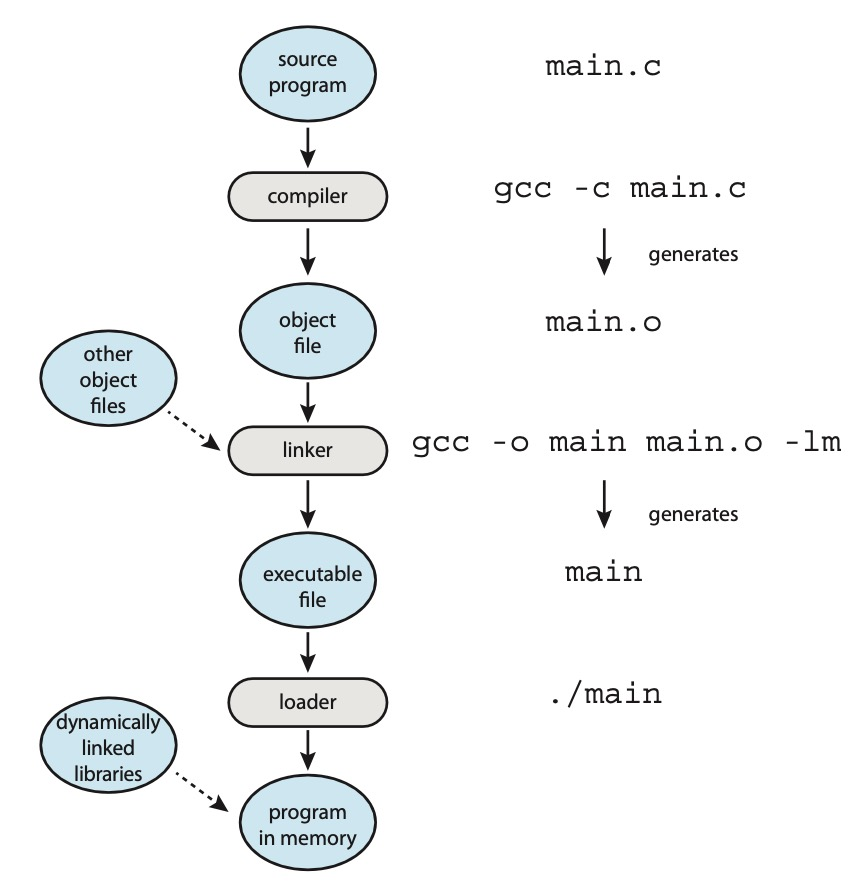
\includegraphics[width=0.38\linewidth]{assets/linker-loader.jpg}
\end{figure}

\begin{note}
    I moderni sistemi operativi \textit{general purpose} non compilano le librerie nei file eseguibili, utilizzano piuttosto delle librerie collegate dinamicamente (es. DLL per Windows) secondo le necessità e condivise da tutti i programmi.
\end{note}

\subsubsection{Le applicazioni sono OS-specific}
Le applicazioni compilate per un sistema \textbf{non} possono, in generale, essere eseguite su altri sistemi. Se questo fosse possibile non dovremmo scegliere il sistema operativo in base agli applicativi che sono disponibili, ma in base alle funzionalità del sistema.

\spacer
Parte del problema, che rende difficile l'interoperabilità tra sistemi, è che ognuno ha il suo \textbf{set di chiamate} a sistema, i propri formati di file eseguibili, ...

\spacer
Ci sono alcune soluzioni per scrivere codice che può essere eseguito su più sistemi:
\begin{itemize}
    \item Scrivere in un \textbf{linguaggio interpretato}, come Python, in questo caso è sufficiente che esista un interprete disponibile per quel sistema operativo.

    \item Scrivere in un linguaggio che \textbf{include una VM} all'interno della quale avviene l'esecuzione, come Java.

    \item Scrivere in un \textbf{linguaggio standard}, come C, e compilare poi per ogni sistema.
\end{itemize}

\subsubsection{ABI}
Proprio come le API permettono al programmatore di non dover programmare le implementazioni di semplici funzioni in codice macchina, le ABI forniscono al compilatore il set di istruzioni che possono essere eseguite sulla specifica architettura per cui si sta compilando.

\spacer
Il problema è che le ABI spesso non forniscono una gran quantità di interoperabilità, quindi il codice deve essere compilato \textbf{per ogni sistema operativo} e \textbf{per ogni architettura} su cui verrà eseguito.
